%%% Document class beamer, do not change
\documentclass[t]{beamer}
%% Optional packages
\usepackage[utf8]{inputenc}
%% Required if you are writing in other language than English
\usepackage[finnish,swedish,english]{babel}
\usepackage{verbatim}
\usepackage{subfig}


%% Input the document information, note the use of short information in the footer
% The document title. Shows an example how linebreaks can be obtained.
\title[Tassu observations]{%
	Tassu observations
}

% The subtitle, e.g. the conference or course name.
% An abbreviation (or similar) in the short version is handy.
\subtitle[S-114.4202]{%
	S-114.4202 Special Course in Computational Engineering II
}
% The author names. Shows a second example of linebreaks.
% Note the use of \inst, see the \institute command!
\author[Väänänen]{%
	Ville Väänänen
}
% The authors' affiliations.
% Note the use of \inst, see the \author command!
\institute[Aalto University School of Science]{%
	Aalto University School of Science
}
% The date. Default date is \today.
%\date[Short Example Date]{%
%	Long Example Date, Default Date is \textbackslash today%
%}
% The subject. This is stored only in the PDF information.
\subject{Document Subject Example}

%\usepackage{mylayout}

% Theme loading
\usetheme{Aalto}

%%% Begin the document
\begin{document}

%%% This file contains the code for the sample0x.tex files.

%% Create the title page
\maketitle

\begin{frame}
	\frametitle{Outline}
	\tableofcontents
	% You might wish to add the option [pausesections]
\end{frame}
\section{Data}

\begin{frame}
	\frametitle{Data}
	\vskip -15pt
	\begin{itemize}
  		\item Wild animal observations in Finland
  		\begin{itemize}
  \item Bear
  \item Wolf
  \item Lynx
  \item Wolverine
	\end{itemize}
  		\item Location (in KKJ coordinates)
  		\item Foot-size measurements
  		\item Date  
	\end{itemize}
	\item{Questions}
	\begin{itemize}
  \item Where the animals really are
  \item Why they are where they are
  \item (How many are there)
\end{itemize}
\end{frame}
	
	
\frame[plain]{
	\vskip -25pt
	\begin{figure}[htb]
		  \centering
		  \subfloat[Bear 2009 (8020)]{\label{fig:b2009}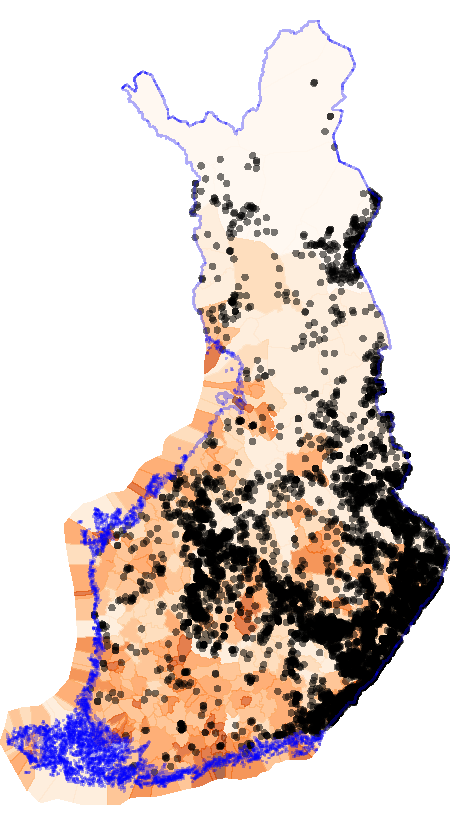
\includegraphics[width=0.4\textwidth]{b2009}}
		  \subfloat[Bear 2010 (10689)]{\label{fig:b2010}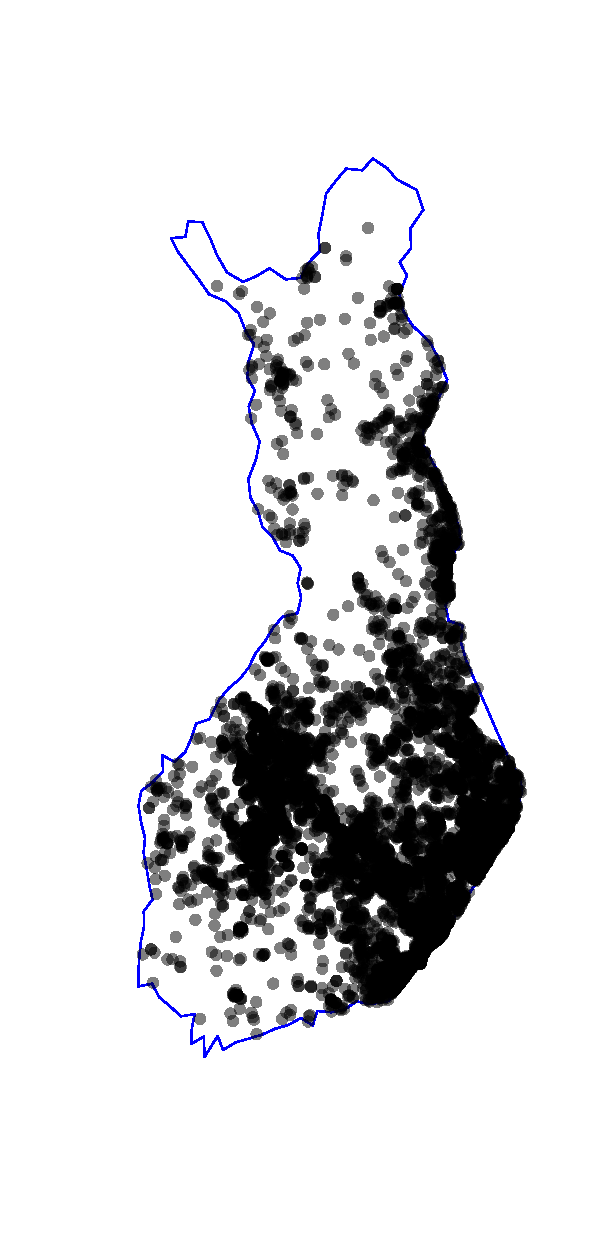
\includegraphics[width=0.4\textwidth]{b2010}}
	  \label{fig:beardata}
	\end{figure}
}
\frame[plain]{
	\vskip -25pt
	\begin{figure}[htb]
		  \centering
		  \subfloat[Lynx 2009 (22682)]{\label{fig:l2009}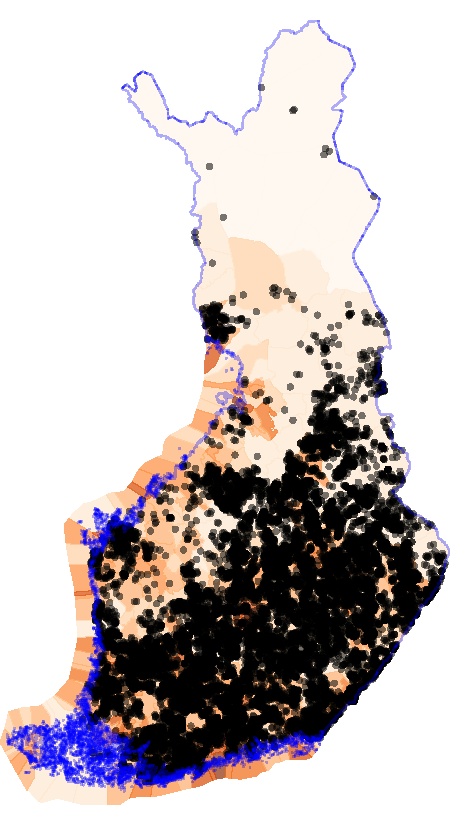
\includegraphics[width=0.4\textwidth]{l2009}}
		  \subfloat[Wolf 2009 (4742)]{\label{fig:w2010}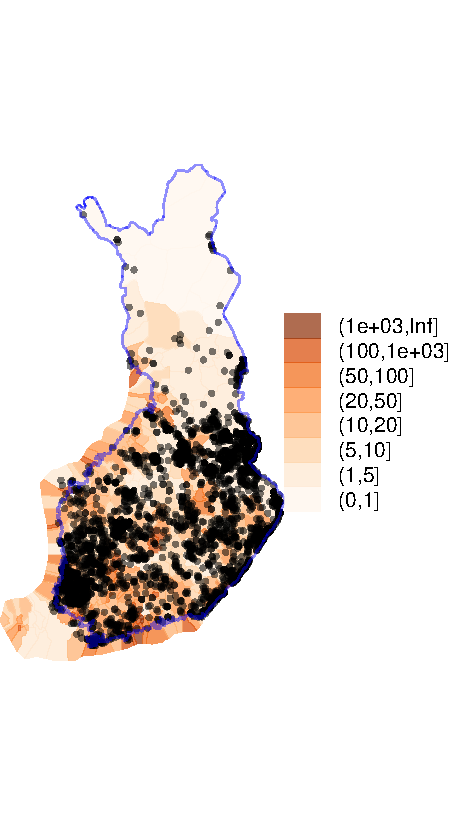
\includegraphics[width=0.4\textwidth]{w2009}}
	  \label{fig:lynxwolfdata}
	\end{figure}
}


\section{Geographical data in R}


\section{Preparing the observation window}

\begin{frame}
	\frametitle{The observation window}
	\vskip -15pt
	\begin{itemize}
  \item From a map (shapefile with lines) to polygon 
  \item A huge effort
  \item Needed for the mesh 
\end{itemize}
\end{frame}

\frame[plain]{
	%\frametitle{Intensity}
	\vskip -25pt
\begin{figure}[htb]
	  \centering
	  \subfloat{\label{fig:mesh}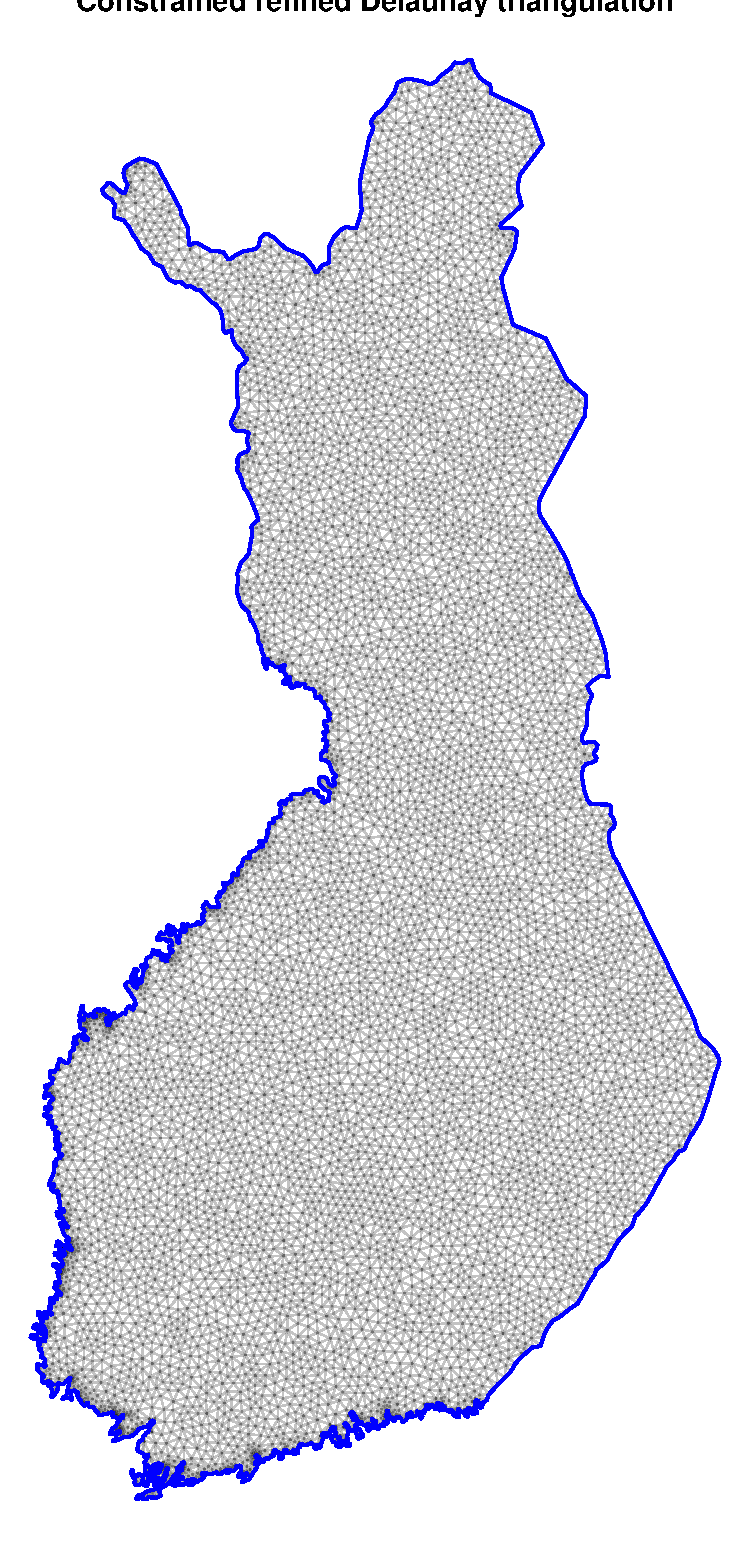
\includegraphics[width=0.4\textwidth]{mesh}}
  	\caption{Mesh}
	  \label{fig:mesh}
\end{figure}
}

\section{Preliminary LGCP fit}

\frame[plain]{
\vskip -60pt
\begin{figure}[htb]
	  \centering
	  \subfloat{\label{fig:bpost}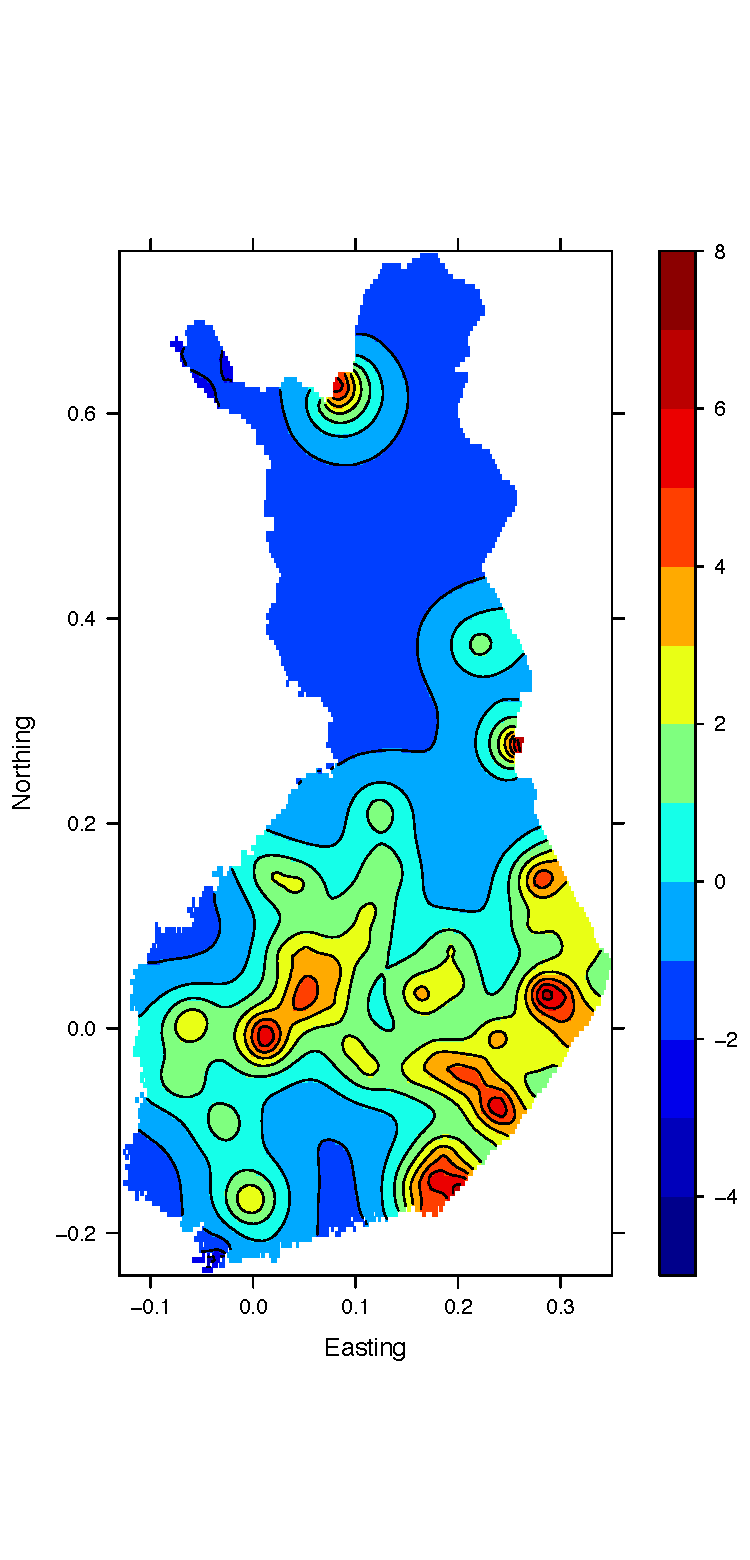
\includegraphics[width=0.55\textwidth]{postint_b2010}}
	  %\subfloat[PPCF]{\label{fig:pcf}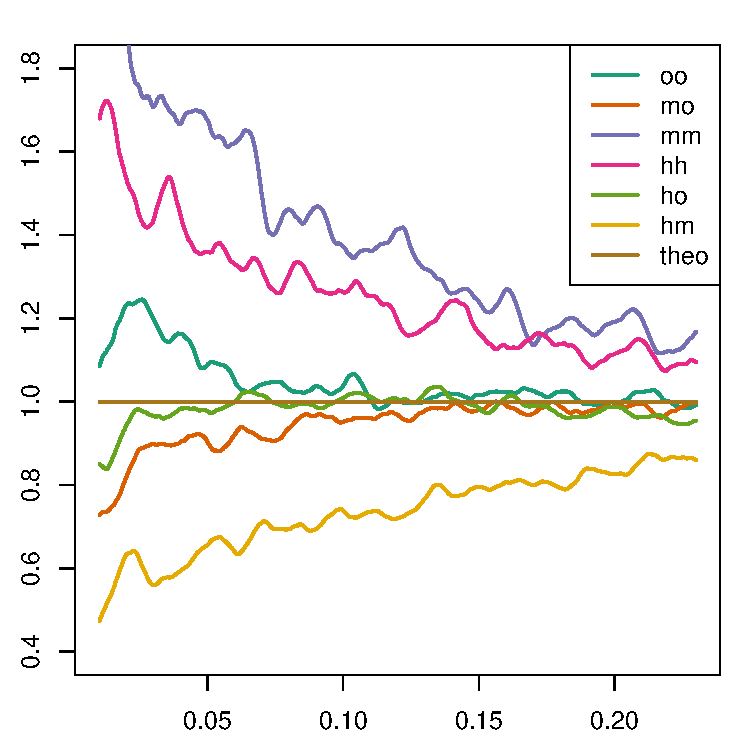
\includegraphics[width=0.52\textwidth]{pcf}}
  \label{fig:postint}
\end{figure}
}

\section{Summary}

\begin{frame}
\frametitle{Summary}

\begin{itemize}
  \item Wild animal observations
  \item Map of Finland as observation window
  \item Tried to fit LGCP using INLA
  \item Covariates: population density  
\end{itemize}

\end{frame}







\end{document}